% Shared manuscript content. Select the review or journal layout through one of
% the two wrapper files in this directory.
\usepackage{array}
\usepackage{booktabs}
\usepackage{calc}
\usepackage{longtable}
\usepackage{graphicx}

\graphicspath{{../../docs/figures/}}
\setlength{\emergencystretch}{2em}
\providecommand{\tightlist}{%
  \setlength{\itemsep}{0pt}\setlength{\parskip}{0pt}}

\acmJournal{TALLIP}
\acmYear{2026}
\setcopyright{none}
\settopmatter{printacmref=false, printfolios=true}
\renewcommand\footnotetextcopyrightpermission[1]{}
\citestyle{acmauthoryear}

\title{When Does LLM-Labeled Silver Data Help?}
\subtitle{An Inductive-Safe Study of Offline Structured Distillation for
Multilingual Dimensional Aspect Sentiment Quad Prediction}

% BEGIN IDENTIFYING METADATA
\author{Hongzhen Qin}
\affiliation{%
  \institution{School of Computer Science and Technology, Hangzhou Dianzi University}
  \city{Hangzhou}
  \postcode{310018}
  \country{China}}
\affiliation{%
  \institution{University of Yamanashi}
  \city{Kofu}
  \country{Japan}}
\email{241050420@hdu.edu.cn}
\email{g24tka12@yamanashi.ac.jp}

\author{Yoshimi Suzuki}
\affiliation{%
  \institution{University of Yamanashi}
  \city{Kofu}
  \country{Japan}}
\email{ysuzuki@yamanashi.ac.jp}

\author{Fumiyo Fukumoto}
\affiliation{%
  \institution{University of Yamanashi}
  \city{Kofu}
  \country{Japan}}
\email{fukumoto@yamanashi.ac.jp}

\author{Renjie Zhou}
\affiliation{%
  \institution{School of Computer Science and Technology, Hangzhou Dianzi University}
  \city{Hangzhou}
  \postcode{310018}
  \country{China}}
\email{rjzhou@hdu.edu.cn}

\renewcommand{\shortauthors}{Qin et al.}
% END IDENTIFYING METADATA

\begin{document}

\begin{abstract}
Large language models (LLMs) can provide labels for a student, removing teacher
cost from deployment. Gains may reflect teacher quality, pool composition,
exposure, split overlap, or development-set selection. This study evaluates
offline structured label distillation for Dimensional Aspect Sentiment Quad
Prediction with a fixed student. Two teachers are evaluated on label-hidden
development sets from eight language--domain datasets; training inputs are
audited for development/test overlap; and five seeds are trained on five
clean-inductive domains. Exposure-matched repeated-gold and same-text
self-training controls test alternatives to LLM supervision, while paired
bootstrap inference, multiplicity correction, and a test lock limit
selection-driven claims. Across the five domains, distillation improves macro
cF1 over the frozen baseline by 0.0600 (95\% CI [0.0291, 0.0911]), over
repeated-gold exposure by 0.0588 [0.0318, 0.0853], and over same-text
self-training by 0.0621 [0.0351, 0.0888]. A reliable per-domain advantage over
self-training is established only for English laptop and Russian restaurant.
DeepSeek leads direct fidelity on all eight datasets, but only three differences
survive Holm correction. One-shot official-test evaluation supports four of
five KD contrasts before correction and three afterward. No universal teacher,
pool, or silver-quantity ranking is supported. Offline LLM supervision is
therefore a conditional tool requiring inductive data hygiene and matched
controls.
\end{abstract}

\ccsdesc[500]{Information systems~Sentiment analysis}
\ccsdesc[500]{Computing methodologies~Information extraction}
\ccsdesc[300]{Computing methodologies~Transfer learning}
\ccsdesc[300]{Computing methodologies~Natural language processing}

\keywords{dimensional aspect-based sentiment analysis, knowledge distillation,
LLM annotation, multilingual NLP, low-resource languages, data contamination,
statistical evaluation}

\maketitle

\section{Introduction}\label{introduction}

Aspect-based sentiment analysis seeks more than a document-level
judgment: it identifies what is being discussed, which property is
evaluated, and how the evaluation is expressed. Aspect Sentiment Quad
Prediction (ASQP) unifies these decisions by predicting aspect terms,
aspect categories, opinion terms, and sentiment polarity as linked
structures rather than independent labels
\citep{cai2021acos,zhang2021asqp}. Dimensional Aspect Sentiment Quad
Prediction (DimASQP) makes the task finer-grained by replacing coarse
polarity with continuous valence and arousal. Its outputs must therefore
be correct both as a set of symbolic structures and as locations in an
affective space. The recent DimABSA resource and SemEval-2026 Task 3
instantiate this problem across six languages and multiple review
domains \citep{lee2026dimabsa,yu2026semeval}. Such coverage is valuable,
but collecting exact spans, long-tailed categories, and calibrated
numerical ratings is expensive, particularly where native annotators or
domain specialists are scarce.

One attractive response is to use an LLM as an offline annotator. Given
an unlabeled in-domain sentence, a teacher can emit a complete
structured label; the resulting \emph{silver} examples are mixed with
human-labeled \emph{gold} examples to train a much smaller student. The
teacher is then absent from inference. This arrangement differs from
serving an LLM directly and from classical logit-transfer distillation:
it uses hard, task-level responses that remain available as ordinary
training data
\citep{hinton2015distilling,hsieh2023distilling,golde2023fabricator}. It
is especially appealing when a compact encoder must run repeatedly or
locally, because the marginal LLM cost is paid during data construction
rather than deployment.

The simplicity of the pipeline hides a difficult evaluation question:
when a student improves, what supplied the improvement? Teacher
annotations may add correct structures that are missing from the gold
set, but teacher fidelity can vary with language, domain, category
inventory, and output schema. A generated, translated, or naturally
occurring text pool can change lexical coverage and label distribution
independently of label quality. More rows also mean more optimizer
exposure even when their labels add no information. A student may
benefit just as much from its own pseudo-labels on the same texts.
Finally, training pools assembled from public or generated sources can
overlap with development or test sentences. Downstream scores alone
confound these mechanisms, while a teacher's direct annotation score
does not guarantee that its errors and coverage are useful to a
particular student \citep{ding2023annotator,zhang2023llmaaa}.

These ambiguities are amplified in a multilingual benchmark with small
development sets. Reusing one development split for encoder selection,
augmentation, checkpointing, thresholds, and ablations invites selection
optimism. Comparing many teachers, pools, datasets, and inference
variants also creates a multiplicity problem. Meanwhile, exact text
leakage can make a nominally inductive result partly transductive. Prior
work has documented both the effects of train--evaluation overlap and
the need for evaluation designs that match the statistical test to
paired NLP outputs \citep{lee2022deduplicating,dror2018hitchhiker}. A
credible silver-data study should therefore audit the data path, measure
teacher behavior directly, construct controls for alternative
explanations, quantify uncertainty, and freeze test decisions before
inspecting held-out labels.

We apply that evidence chain to offline DimASQP distillation. First, we
measure DeepSeek and Qwen on the same label-hidden gold development
sentences for all eight task datasets. Second, we normalize and audit
gold, silver, distillation, development, and test inputs, remove
detected overlap from three adopted training sets, and preserve
deletion-level provenance. Third, we run five student seeds in each of
five adopted KD domains with frozen ensemble rules. For each domain, a
repeated-gold control matches training-row exposure, and a student
self-training control additionally matches the silver texts and row
count. Teacher, pool, and quantity comparisons are separated according
to how well they control the remaining factors. Paired example-level
bootstrap intervals, task-macro effects, Holm family-wise correction,
and Benjamini--Hochberg false-discovery correction make the inferential
scope explicit. Official test predictions and their hashes are fixed
before the released labels are read.

The resulting picture is neither ``silver always helps'' nor ``the
highest-scoring teacher always wins.'' The five-domain macro effect is
positive against the frozen baseline, repeated-gold exposure, and
same-text self-training, but single-domain support is uneven. In the
strongest teacher-source test, only the English laptop and Russian
restaurant gains remain supported after correcting within the
five-domain family. DeepSeek's direct fidelity is numerically higher on
all eight datasets, yet most individual teacher gaps remain uncertain,
and direct fidelity is not a monotonic predictor of downstream gain. The
frozen official-test analysis supports conditional transfer in four
adopted domains before multiplicity correction and three afterward,
while the Chinese restaurant contrast is inconclusive. These results
motivate a narrower and more useful claim: LLM-labeled silver can
improve a fixed structured student on average, but teacher identity,
pool source, and sample count are insufficient universal selection
rules.

Our contributions are fourfold:

\begin{enumerate}
\def\labelenumi{\arabic{enumi}.}
\tightlist
\item
  We formulate an offline structured LLM-to-student distillation
  protocol for multilingual DimASQP while keeping the previously
  introduced student and inference procedure fixed.
\item
  We directly evaluate two teachers on eight label-hidden development
  sets and disentangle teacher, pool, quantity, exposure, and same-text
  pseudo-label effects through matched controls.
\item
  We provide an inductive-safe and multiplicity-aware evaluation with
  five seeds, paired bootstrap inference, deletion-level provenance, and
  frozen official-test decision rules.
\item
  We show reliable average gains but substantial domain heterogeneity,
  and identify the limits of teacher fidelity, pool source, and silver
  quantity as universal selection rules.
\end{enumerate}

\section{Related Work}\label{related-work}

\subsection{Structured and Dimensional Aspect-Based Sentiment
Analysis}\label{structured-and-dimensional-aspect-based-sentiment-analysis}

Aspect-based sentiment analysis has progressed from predicting
individual sentiment elements to extracting their relations jointly.
ACOS quadruple extraction explicitly includes aspect, category, opinion,
and categorical sentiment, including implicit aspects and opinions
\citep{cai2021acos}. ASQP casts the same linked prediction problem as
conditional generation, showing the appeal of end-to-end structured
output over pipelines whose errors propagate between subtasks
\citep{zhang2021asqp}. Both formulations retain discrete sentiment
polarity.

DimABSA instead represents sentiment with continuous valence--arousal
ratings and provides multilingual, multidomain annotations that combine
these ratings with traditional ABSA elements \citep{lee2026dimabsa}.
SemEval-2026 Task 3 defines regression, triplet, and quadruplet subtasks
and introduces continuous F1 to combine structural correctness with
valence--arousal error \citep{yu2026semeval}. Participating systems span
encoder-based extraction, instruction-tuned generation, hybrid
pipelines, and ensembling. Some also use LLMs or LLM-generated
annotations, establishing the practical relevance of generated
supervision but not, by itself, separating annotation quality from pool
or selection effects \citep{alshawi2026classics}.

The earlier ICONIP work introduced the LEADER-DimASQP student,
dataset-specific encoder and training recipes, and five-seed inference
\citep{qin2026leader}. The present paper does not re-claim those
architectural components. It fixes them as experimental infrastructure
and studies whether, when, and why LLM-labeled training examples improve
that student. This separation is important because architecture
selection and supervision-source selection otherwise share the same
development signal.

\subsection{Distillation, Pseudo-Labeling, and LLM-Generated
Supervision}\label{distillation-pseudo-labeling-and-llm-generated-supervision}

Knowledge distillation traditionally compresses the predictive behavior
of a large teacher into a smaller student, often through softened output
distributions \citep{hinton2015distilling}. Pseudo-labeling and
self-training instead use a model's hard predictions as targets on
unlabeled inputs \citep{lee2013pseudolabel}. The two ideas overlap
operationally but answer different questions: classical KD asks how to
transfer a teacher's predictive knowledge, whereas self-training asks
whether a learner can exploit additional unlabeled examples using its
own decisions.

LLMs broaden response-based distillation because their textual outputs
can become labels, rationales, or complete generated datasets.
Distilling step-by-step uses LLM-produced rationales as additional
supervision for smaller models, and other work studies cost-aware
transfer or tool support for creating labeled data with teacher LLMs
\citep{hsieh2023distilling,dasgupta2023cost,golde2023fabricator}. LLMaAA
incorporates LLM annotation into an active-learning loop and reweights
noisy pseudo-labels, demonstrating that student utility depends on
annotation and training design rather than teacher size alone
\citep{zhang2023llmaaa}.

Our setting uses neither teacher logits nor rationales. The teacher
emits hard DimASQP structures constrained by the task schema, and the
student trains on the accepted rows together with its inherited
gold/base data. We therefore use \emph{offline structured label
distillation} to distinguish the protocol from logit-based compression,
direct LLM inference, and pure text augmentation. We also compare LLM
labels with two controls that standard KD reports often omit: repeated
gold matches row exposure, while student pseudo-labels on the identical
silver texts ask whether the LLM is adding label information beyond
ordinary self-training.

\subsection{LLM Annotation in Multilingual and Low-Resource
Settings}\label{llm-annotation-in-multilingual-and-low-resource-settings}

LLMs are attractive annotators because one interface can scale across
tasks and reduce the amount of manual labeling. Broad evaluations have
examined their fitness as general-purpose annotators, while human--LLM
allocation methods use uncertainty to reserve difficult examples for
people \citep{ding2023annotator,li2023coannotating}. These studies also
caution against treating syntactic validity or aggregate accuracy as a
substitute for task-specific reliability. For structured DimASQP, a
response can be valid JSON yet still omit an opinion, misplace a span
boundary, choose a frequent category, or miscalibrate the
valence--arousal scale.

Multilingual annotation adds another layer of variation. Evidence from
low-resource classification shows that strong LLM annotators can lag
task-specific models outside high-resource languages
\citep{jadhav2025limitations}. Annotation instructions, model
disagreement, cultural context, and language imbalance can also
introduce systematic annotation bias \citep{cui2025bias}. Resource level
alone does not determine the direction of that effect: domain
vocabulary, category inventories, few-shot examples, and the student's
representation all matter.

We consequently avoid equating a low-resource language with a large
expected KD gain. Our teacher-fidelity experiment hides the gold labels
and sends the same examples to both teachers in each of eight datasets.
It reports not only the official cF1 but structural components,
matched-quad numerical errors, invalid responses, empty outputs,
\texttt{NULL} behavior, and rare-category coverage. The downstream
matched-text control then asks a separate question: even when two label
sources see identical texts, does the LLM supervision improve the fixed
student? Keeping these two levels separate prevents student accuracy
from being used as a proxy for teacher annotation quality.

\subsection{Leakage-Aware and Statistical Evaluation of Silver
Data}\label{leakage-aware-and-statistical-evaluation-of-silver-data}

Silver-data experiments are vulnerable to leakage at several stages.
Public or generated pools may duplicate development/test text, and
benchmark material may also enter opaque model pretraining.
Deduplication research shows that train--evaluation overlap can inflate
measured performance and bias selection \citep{lee2022deduplicating}.
Contamination audits have further shown that the problem extends across
benchmarks and can cross language boundaries
\citep{sainz2024contamination,yao2024crosslingual}. Our audit cannot
determine the unknown pretraining contents of proprietary teachers. It
addresses the controllable leakage path instead: every registered
training-side source is checked against the task development and test
splits by exact text, normalized text, and source identifier, with every
deletion and file hash retained.

Evaluation also needs to respect paired outputs and repeated
comparisons. Bootstrap resampling provides a practical way to estimate
uncertainty for nonlinear corpus metrics, and NLP-specific guidance
emphasizes selecting tests that match the task and experimental design
\citep{koehn2004statistical,dror2018hitchhiker}. Once results are
inspected across multiple datasets or contrasts, unadjusted significance
statements no longer control the probability of false positives. Holm's
sequential procedure controls the family-wise error rate, while
Benjamini--Hochberg controls the false discovery rate under its stated
conditions \citep{holm1979,benjamini1995}.

Our protocol combines these ideas in an audit-and-freeze design. We use
paired example-level bootstrap intervals and p-values, group comparisons
into declared families for multiplicity correction, and report an
equal-weight fixed-task macro effect without converting it into a
universal language claim. Most importantly, the released official test
labels are accessed only after systems, thresholds, predictions, and
hashes are frozen. The test evaluation can then check whether a
development conclusion transfers; it cannot become a new source for
teacher, pool, augmentation, or threshold selection.

\section{Task and Offline Structured
Distillation}\label{task-and-offline-structured-distillation}

\subsection{Dimensional Aspect Sentiment Quad
Prediction}\label{dimensional-aspect-sentiment-quad-prediction}

Given an input sentence \(x=(x_1,\ldots,x_n)\), the Dimensional Aspect
Sentiment Quad Prediction (DimASQP) task requires a system to predict an
unordered set

\[
Y=\{(a_i,c_i,o_i,V_i,A_i)\}_{i=1}^{m},
\]

where \(a_i\) is an aspect span or \texttt{NULL}, \(o_i\) is an opinion
span or \texttt{NULL}, and \(c_i\) is an entity--attribute category
defined by the dataset. The two continuous labels \(V_i,A_i\in[1,9]\)
represent valence and arousal, respectively. A sentence can contain no
opinion, one opinion, or multiple opinions; the cardinality \(m\) is
therefore unknown at prediction time.
\citep{lee2026dimabsa,yu2026semeval}

We use the official Task-3 continuous F1 (cF1) as the primary metric. A
predicted quad is eligible for matching when its categorical triple
\((a,c,o)\) matches a gold triple. For each matched pair, the continuous
true positive credit is

\[
\operatorname{cTP}
=1-\frac{\sqrt{(V_p-V_g)^2+(A_p-A_g)^2}}{\sqrt{2(9-1)^2}}.
\]

Continuous precision and recall replace the ordinary true-positive count
with the sum of this credit, and cF1 is their harmonic mean. The metric
consequently penalizes both structural extraction errors and inaccurate
valence--arousal estimates. We compute all primary scores with the
official evaluator. For teacher diagnosis, we additionally report exact
categorical F1; aspect, opinion, and category F1; valence--arousal mean
absolute error and root mean squared error on matched quads; and
coverage for \texttt{NULL}, rare categories, empty outputs, and invalid
outputs.

\subsection{Fixed Student Model}\label{fixed-student-model}

The experiments build on the LEADER-DimASQP student introduced in an
earlier ICONIP study \citep{qin2026leader}. We treat that model and its
dataset-specific training recipes as inherited experimental
infrastructure rather than as a new contribution of the present work.
Fixing the student is essential here: the object of study is the
supervision supplied by LLM-labeled silver data, not a new extraction
architecture.

In brief, the student encodes the sentence and predicts aspect and
opinion BIO spans. It forms candidate aspect--opinion pairs and uses
task-specific heads to predict pair validity, entity and attribute
labels, and continuous valence and arousal. A lightweight Rethink stage
embeds the draft span, category, and valence--arousal predictions and
fuses them back into the token representations. Candidate quads are
aligned with gold quads through Hungarian set matching. The inherited
training recipes also use mild fast-gradient adversarial perturbations
and an exponential moving average. At inference, five independently
trained students vote on the categorical triple; retained quads carry
the corresponding continuous predictions.

We preserve the encoder and optimization recipe selected for each
dataset in the prior study. The five adopted distillation settings use
DeBERTa-v3-base for English laptop, XLM-R-large for Russian and Tatar
restaurant, mDeBERTa-v3-base for Ukrainian restaurant, and Chinese
RoBERTa-wwm-ext-large for Chinese restaurant. No architecture component,
encoder, or inference rule is selected using the experiments reported in
this paper.

\subsection{Offline Structured Label
Distillation}\label{offline-structured-label-distillation}

Let \(G_d\) denote the labeled training data for dataset \(d\), and let
\(U_d\) be an unlabeled text pool from the same task domain. An LLM
teacher \(t\) maps each \(u\in U_d\) to a set of structured DimASQP
labels. The prompt requires non-\texttt{NULL} aspects and opinions to be
verbatim substrings of the input, restricts categories to the inventory
derived from \(G_d\), constrains valence and arousal to \([1,9]\), and
permits an empty set when the sentence contains no in-domain opinion.
Responses are parsed into the task JSON schema, and accepted examples
form the silver set \(S_{d,t}\). The student is then trained on

\[
T_{d,t}=G_d\cup S_{d,t}.
\]

This is response-based structured distillation: the teacher supplies
hard structured labels rather than logits, hidden states, or token-level
probabilities. The LLM is used only while constructing \(S_{d,t}\).
Validation, official-test evaluation, and deployment use the student
checkpoints alone and make no teacher calls.

The adopted systems cover five datasets and were fixed before
official-test labels were inspected. Table 1 records the supervision
actually used after the inductive audit. The ``gold/base'' column
includes the inherited non-silver training recipe, which can contain
training-only augmentation from the prior system; it is therefore not
always equal to the raw gold-train size.

{\small
\begin{longtable}[]{@{}
  >{\raggedright\arraybackslash}p{(\linewidth - 14\tabcolsep) * \real{0.1200}}
  >{\raggedright\arraybackslash}p{(\linewidth - 14\tabcolsep) * \real{0.1800}}
  >{\raggedright\arraybackslash}p{(\linewidth - 14\tabcolsep) * \real{0.1200}}
  >{\raggedright\arraybackslash}p{(\linewidth - 14\tabcolsep) * \real{0.1800}}
  >{\raggedleft\arraybackslash}p{(\linewidth - 14\tabcolsep) * \real{0.1100}}
  >{\raggedleft\arraybackslash}p{(\linewidth - 14\tabcolsep) * \real{0.1000}}
  >{\raggedleft\arraybackslash}p{(\linewidth - 14\tabcolsep) * \real{0.1000}}
  >{\raggedleft\arraybackslash}p{(\linewidth - 14\tabcolsep) * \real{0.0900}}@{}}
\caption{Adopted offline-distillation settings after inductive cleaning.}
\label{tab:adopted-settings}\\
\toprule
Dataset & Fixed encoder & LLM teacher & Silver pool & Gold/base rows &
Silver rows & Total rows & Vote \\
\midrule
\endfirsthead
\caption[]{Adopted offline-distillation settings after inductive cleaning
(continued).}\\
\toprule
Dataset & Fixed encoder & LLM teacher & Silver pool & Gold/base rows &
Silver rows & Total rows & Vote \\
\midrule
\endhead
\bottomrule
\endlastfoot
English laptop & DeBERTa-v3-base & DeepSeek V4 Pro & existing in-domain
pool & 15,048 & 7,547 & 22,595 & 4 \\
Russian restaurant & XLM-R-large & DeepSeek V4 Pro & native generation,
gen4k batch & 1,240 & 3,000 & 4,240 & 3 \\
Tatar restaurant & XLM-R-large & Qwen3.6-35B & native generation & 1,240
& 3,915 & 5,155 & 3 \\
Ukrainian restaurant & mDeBERTa-\allowbreak v3-base & DeepSeek V4 Pro & translated
construction & 2,966 & 5,534 & 8,500 & 3 \\
Chinese restaurant & Chinese RoBERTa-\allowbreak wwm-\allowbreak ext-large & DeepSeek V4 Pro &
real-text pool & 6,050 & 3,882 & 9,932 & 3 \\
\end{longtable}
}

The choices in Table 1 are not claims of a universally optimal teacher
or pool. They are the frozen adopted systems whose behavior we audit.
Separate matched experiments vary teacher identity, pool source, or
silver quantity while holding the remaining observable factors fixed
when the available data permit such a comparison.

\subsection{Experimental Factors and Competing
Explanations}\label{experimental-factors-and-competing-explanations}

We distinguish four factors that are often conflated in silver-data
studies. First, \textbf{teacher fidelity} measures whether an LLM can
directly reproduce hidden gold labels. Second, \textbf{pool source}
describes where the unlabeled text comes from: native generation, real
public text, or machine translation. Third, \textbf{silver quantity} is
the number of accepted silver rows. A comparison between independently
generated batches changes both quantity and batch composition, whereas a
cap applied to one fixed pool changes quantity while preserving the
underlying source. Fourth, \textbf{information complementarity}
describes whether silver supervision supplies valid categories, spans,
or error corrections that are underrepresented in the base training
data.

A higher downstream score alone cannot identify which factor is
responsible. It may also reflect more optimizer updates, a favorable
random seed, train--test text overlap, or labels that the student could
have produced itself. We therefore combine direct teacher evaluation
with inductive cleaning, five-seed training, exposure-matched
repeated-gold controls, same-text student self-training controls, and
paired inference on frozen predictions.

\section{Experimental Design}\label{experimental-design}

\subsection{Datasets and Evaluation
Roles}\label{datasets-and-evaluation-roles}

We study all eight datasets from SemEval-2026 Task 3
\citep{yu2026semeval}. They span English, Japanese, Russian, Tatar,
Ukrainian, and Chinese, with laptop, restaurant, and hotel domains.
Table 2 reports the raw gold split sizes. All eight datasets participate
in direct teacher-fidelity evaluation. Five datasets---English laptop
and the Russian, Tatar, Ukrainian, and Chinese restaurant sets---have a
frozen adopted KD system and enter the matched downstream analyses.
English restaurant, Japanese hotel, and Chinese laptop retain their
inherited non-KD main systems and are not silently counted as KD
successes.

{\small
\begin{longtable}{@{\extracolsep{\fill}}lrrrcc@{}}
\caption{Gold data and evaluation roles. Language and domain are encoded in
the dataset identifiers.}
\label{tab:data-roles}\\
\toprule
Dataset & Train & Dev & Test & Direct fidelity & Adopted KD \\
\midrule
\endfirsthead
\toprule
Dataset & Train & Dev & Test & Direct fidelity & Adopted KD \\
\midrule
\endhead
\bottomrule
\endlastfoot
eng\_laptop     & 4,076 & 200 & 1,000 & yes & yes \\
eng\_restaurant & 2,284 & 200 & 1,000 & yes & no  \\
jpn\_hotel       & 1,600 & 200 &   800 & yes & no  \\
rus\_restaurant & 1,240 &  48 &   630 & yes & yes \\
tat\_restaurant & 1,240 &  48 &   630 & yes & yes \\
ukr\_restaurant & 1,240 &  48 &   630 & yes & yes \\
zho\_laptop      & 3,490 & 300 & 1,000 & yes & no  \\
zho\_restaurant & 6,050 & 300 & 1,000 & yes & yes \\
\end{longtable}}

The development sets serve two distinct roles. Their labels are hidden
from the LLMs when directly measuring teacher fidelity, while the
student experiments use development cF1 for the inherited
validation-based checkpoint rule. The released official test labels are
reserved for a single post-competition local evaluation after systems,
thresholds, prediction files, and hashes have been locked.

\subsection{Contamination Audit and Inductive
Cleaning}\label{contamination-audit-and-inductive-cleaning}

We audit the gold, pool, silver, combined distillation, development, and
test files registered for all eight datasets. Each training-side row is
checked against development and test by exact text, normalized text, and
source ID. The normalization key applies Unicode NFKC normalization,
Unicode case folding, and Unicode-whitespace collapse. The audit stores
the source path, source SHA-256, line number, matched split, match
reason, and normalized text for each detected row.

Three adopted KD inputs contain development- or test-overlapping text
and are filtered without reordering the retained rows. English laptop
changes from 23,590 to 22,595 rows, Ukrainian restaurant from 9,105 to
8,500, and Chinese restaurant from 10,911 to 9,932. The corresponding
English and Ukrainian baseline inputs each contain one normalized
development overlap and are also cleaned, from 15,049 to 15,048 rows and
from 2,967 to 2,966 rows, respectively. The Russian gen4k and Tatar Qwen
adopted inputs have zero normalized overlap and are retained unchanged.
We then verify that every final adopted KD input and every baseline
input used for a clean paired comparison has zero normalized text
overlap with development and test. Original checkpoints are preserved;
clean runs use distinct prefixes.

This cleaning step defines the inductive protocol and is not conditioned
on whether removal raises or lowers cF1. We report comparisons with the
earlier transductive checkpoints only to quantify sensitivity, never as
evidence that overlap would have been acceptable.

\subsection{Direct Teacher-Fidelity
Evaluation}\label{direct-teacher-fidelity-evaluation}

We evaluate DeepSeek V4 Pro and Qwen3.6-35B directly on every gold
development set. We remove the complete \texttt{Quadruplet} field before
sending an example to a teacher. The category inventory and six few-shot
demonstrations are drawn only from that dataset's training split. Both
teachers receive prompt version \texttt{dim-asqp-fidelity-v1},
temperature 0.3, and disabled reasoning output. A 10-example smoke run
checks model identity, schema compatibility, and output coverage before
a full run is accepted.

Across the eight datasets, the development sets contain 1,344 examples.
Each teacher produces exactly one validated record for every example,
giving 1,344 DeepSeek and 1,344 Qwen annotations with zero final error
rows. We retain the label-free inputs, raw responses, parsed outputs,
requested and returned model names, prompt version, temperature,
timestamps, and SHA-256 hashes. The main fidelity metric is official
cF1. The auxiliary metrics defined in Section 3.1 diagnose whether a
difference comes from structure, category, continuous sentiment, empty
output, or an infrequent training category. A category is treated as
rare for this diagnostic when it appears no more than five times in the
corresponding training split.

Direct fidelity does not by itself establish which teacher produces the
best training signal. To test whether a downstream teacher ranking can
be reproduced under matched conditions, we additionally train Tatar
students on the same 1,240 gold rows and the same 3,915 silver texts in
the same order, changing only whether DeepSeek or Qwen supplies the
silver labels. Both arms use all five seeds and the same frozen
inference threshold.

\subsection{Student Training and Frozen
Inference}\label{student-training-and-frozen-inference}

Every five-seed experiment uses random seeds 42, 123, 456, 789, and
1024. We inherit the dataset-specific model configuration, optimizer,
training data order, augmentation recipe, maximum of 30 epochs,
validation-based checkpoint selection, and early-stopping patience of
eight from the corresponding fixed student. The adopted configurations
use AdamW, an encoder learning rate of \(1.5\times10^{-5}\), a warmup
ratio of 0.1, weight decay 0.01, gradient-norm clipping at 1.0, FGM with
\(\epsilon=0.1\), and EMA with decay 0.999. Batch size is eight for the
base-size English and Ukrainian encoders and four for the large Russian,
Tatar, and Chinese encoders. We retain and evaluate
\texttt{checkpoint\_best.pt}; no last-epoch checkpoint is substituted.

For the clean-inductive reruns, the only intended experimental change is
the removal of overlapping rows. The five-seed ensemble thresholds are
fixed at vote 4 and top-k 0 for English laptop, and vote 3 and top-k 0
for Russian, Tatar, Ukrainian, and Chinese restaurant. The matched
baseline can retain its own previously fixed threshold; thresholds are
not re-swept to favor a contrast. We report every single-seed cF1, the
mean and sample standard deviation across seeds, and the frozen ensemble
cF1.

\subsection{Controls for Exposure and Teacher
Source}\label{controls-for-exposure-and-teacher-source}

The \textbf{repeated-gold control} tests whether a gain can be explained
by seeing more training rows or performing more updates. For each
adopted KD dataset, we repeat the inductive-safe base training rows as
evenly as possible until the control has exactly the same number of rows
as the corresponding gold-plus-LLM training input. Complete copies
preserve source order; a remainder is selected after a deterministic
shuffle with seed 20260713. Duplicate copies receive unique IDs. Each
constructed file must have zero normalized overlap with development and
test, and it is trained with the same student recipe and five seeds as
the adopted KD arm.

The \textbf{same-text self-training control} tests the value of LLM
labels rather than the value of the unlabeled text itself. We extract
exactly the silver-text tail used by an adopted LLM arm, preserve its
IDs and order, and remove its labels. A five-seed ensemble trained on
the repeated-gold control then labels those texts. We combine the
inductive-safe base rows with the resulting student pseudo-labels,
retaining empty predictions as valid no-quad pseudo-labels. The final
self-training input therefore has the same base rows, the same silver
texts, the same silver row count, and the same total row count as the
LLM arm; the supervision source on the silver texts is the intended
difference. It is trained with the same five seeds and evaluated using
the adopted system's frozen threshold.

All exposure and self-training controls were registered after the
official-test systems had been locked. They use development data only,
and their manifests explicitly forbid official-test evaluation.
Consequently, they refine the mechanistic interpretation of the
development results but cannot retrospectively alter any main-system or
test choice.

\subsection{Teacher, Pool, and Quantity
Ablations}\label{teacher-pool-and-quantity-ablations}

We organize auxiliary ablations by the strength of their control. The
direct 8-by-2 fidelity experiment compares teachers on identical
label-hidden inputs. The Tatar downstream experiment compares teachers
on identical gold and silver texts. For Russian pool source, real,
translated, and generated text is labeled by the same teacher and capped
at 3,000 rows. The Chinese real-versus-generated comparison is retained
as observational evidence because other construction details are not
fully matched.

Quantity is evaluated separately from pool identity. In Russian, we take
the same gen8k silver pool and compare a cap of 3,000 with all 7,988
rows for paired seeds 42 and 123. A preregistered gate required the
two-seed mean to improve by at least 1.5 percentage points before
training the remaining seeds or adding a 5,000-row arm. The gate failed,
so the remaining quantity curve was not run. This stopping rule can test
whether the earlier gen4k advantage is explained by having fewer rows;
it cannot identify a universal optimal silver dose.

\subsection{Paired Inference, Macro Effects, and
Multiplicity}\label{paired-inference-macro-effects-and-multiplicity}

For a comparison between systems (A) and (B), we resample evaluation
examples with replacement, recompute both cF1 scores from the
corresponding row-level sufficient statistics, and record
\(\Delta=\operatorname{cF1}_A-
\operatorname{cF1}_B\). Every paired bootstrap uses 10,000 resamples and
random seed 20260713. We report the observed delta, percentile 95\%
confidence interval, and two-sided bootstrap p-value. An interval whose
lower bound is above zero is classified as supported improvement; an
interval that crosses zero is inconclusive; and an interval whose upper
bound is below zero supports harm. An inconclusive interval is not
interpreted as equivalence.

To summarize the five adopted datasets without allowing the larger
English or Chinese evaluation sets to dominate, we also use a fixed-task
macro bootstrap. Examples are resampled independently within each
dataset, a paired delta is recomputed, and the five dataset deltas
receive equal weight. This estimand is the macro-average effect over the
fixed adopted-domain set, not an estimate for unobserved languages or
tasks.

We treat teacher fidelity, adopted KD versus baseline, exposure control,
same-text self-training, self-training versus repeated gold, and frozen
official-test comparisons as separate families. Within each family, we
report both Holm family-wise-error correction and Benjamini--Hochberg
false-discovery correction. The official-test correction is a post-hoc
robustness analysis and does not change the previously frozen systems.
Dataset-level confidence intervals remain visible so that aggregate
support cannot be misread as support for every domain.

\subsection{Official-Test Lock and
Reproducibility}\label{official-test-lock-and-reproducibility}

The official-test evaluation is a one-shot, post-competition local
analysis of the released Task-3 labels. Before obtaining those labels,
we fixed each main system, comparison baseline, five-seed checkpoint
set, vote and top-k threshold, test input, prediction file, row count,
and SHA-256 hash in a protocol manifest. All selections were based on
development evidence. Test labels were not used to choose a checkpoint,
teacher, pool, augmentation recipe, threshold, or stopping rule. We
therefore describe these scores as a frozen local evaluation, not as a
new shared-task submission.

The reproducibility package retains the contamination matches and
deletion records, clean-file hashes, teacher inputs and raw responses,
validated outputs, training and inference manifests, seed-level
predictions, best-checkpoint provenance, bootstrap seed, and
exact-repeat audit. Automated checks verify that teacher inputs contain
no \texttt{Quadruplet}, each input ID has one output or an explicit
error record, final adopted training inputs have zero normalized
development/test overlap, inference uses \texttt{checkpoint\_best.pt},
frozen ensemble thresholds are respected, and the six core evidence
tables match their locked hashes.

Post-lock control training was run on a single 24-GB NVIDIA RTX 4090.
LLMs are offline annotators only, so student inference makes zero LLM
calls. Historical provider token counts and monetary billing were not
retained; we report them as unavailable rather than reconstructing a
potentially misleading cost estimate.

\section{Results}\label{results}

\subsection{Direct Fidelity Favors DeepSeek Overall, but Most Pairwise
Differences Remain
Uncertain}\label{direct-fidelity-favors-deepseek-overall-but-most-pairwise-differences-remain-uncertain}

Table 3 reports teacher fidelity when the complete development labels
are hidden. DeepSeek obtains the higher cF1 point estimate on all eight
datasets, but the size and certainty of the difference vary
substantially. The paired 95\% interval excludes zero for English
restaurant, Chinese laptop, and Chinese restaurant only; these same
three comparisons remain significant after Holm and Benjamini--Hochberg
correction within the eight-dataset family. The other five comparisons
are inconclusive rather than evidence of equivalence.

{\small
\begin{longtable}[]{@{}
  >{\raggedright\arraybackslash}p{(\linewidth - 10\tabcolsep) * \real{0.1364}}
  >{\raggedleft\arraybackslash}p{(\linewidth - 10\tabcolsep) * \real{0.1818}}
  >{\raggedleft\arraybackslash}p{(\linewidth - 10\tabcolsep) * \real{0.1818}}
  >{\raggedleft\arraybackslash}p{(\linewidth - 10\tabcolsep) * \real{0.1818}}
  >{\raggedleft\arraybackslash}p{(\linewidth - 10\tabcolsep) * \real{0.1818}}
  >{\raggedright\arraybackslash}p{(\linewidth - 10\tabcolsep) * \real{0.1364}}@{}}
\caption{Direct teacher fidelity on label-hidden gold development data.}
\label{tab:teacher-fidelity}\\
\toprule
Dataset & DeepSeek cF1 & Qwen cF1 & DS$-$Qwen & 95\% CI & Decision \\
\midrule
\endfirsthead
\caption[]{Direct teacher fidelity on label-hidden gold development data
(continued).}\\
\toprule
Dataset & DeepSeek cF1 & Qwen cF1 & DS$-$Qwen & 95\% CI & Decision \\
\midrule
\endhead
\bottomrule
\endlastfoot
eng\_\allowbreak laptop & 0.3575 & 0.3170 & +0.0404 & {[}−0.0066, +0.0879{]} &
inconclusive \\
eng\_\allowbreak restaurant & 0.5529 & 0.3638 & +0.1892 & {[}+0.1418, +0.2384{]} &
supported \\
jpn\_\allowbreak hotel & 0.2146 & 0.2004 & +0.0142 & {[}−0.0344, +0.0610{]} &
inconclusive \\
rus\_\allowbreak restaurant & 0.3904 & 0.3649 & +0.0255 & {[}−0.0494, +0.1039{]} &
inconclusive \\
tat\_\allowbreak restaurant & 0.4359 & 0.3954 & +0.0405 & {[}−0.0675, +0.1516{]} &
inconclusive \\
ukr\_\allowbreak restaurant & 0.3786 & 0.3598 & +0.0188 & {[}−0.0579, +0.0879{]} &
inconclusive \\
zho\_\allowbreak laptop & 0.2821 & 0.2374 & +0.0447 & {[}+0.0137, +0.0755{]} &
supported \\
zho\_\allowbreak restaurant & 0.4653 & 0.4060 & +0.0593 & {[}+0.0240, +0.0941{]} &
supported \\
\end{longtable}
}

Direct fidelity and downstream student performance need not induce the
same ranking. On the Tatar matched-text control, the DeepSeek-labeled
arm reaches 0.5365 ensemble cF1 and the Qwen-labeled arm reaches 0.5327.
Their difference is only +0.0038 with a 95\% CI of
{[}−0.0823,+0.0852{]}. On the frozen official test, the matched
DeepSeek−Qwen difference is likewise positive but inconclusive at
+0.0109 {[}−0.0069,+0.0293{]}. Thus, the earlier observation that one
Qwen student scored higher under a different run does not establish a
reliable Tatar teacher-ranking reversal.

\subsection{Clean-Inductive KD Has a Positive Macro Effect and
Heterogeneous Domain
Effects}\label{clean-inductive-kd-has-a-positive-macro-effect-and-heterogeneous-domain-effects}

All five adopted systems remain operational after the inductive audit.
Table 4 shows the five individual seed scores, their mean and sample
standard deviation, the frozen ensemble, and the paired ensemble
contrast with its matched baseline. English and Russian show supported
development improvements. Tatar, Ukrainian, and Chinese restaurant have
positive point estimates but intervals that cross zero. After Holm
correction within the five-domain baseline family, only the English
comparison remains significant; English and Russian remain significant
under Benjamini--Hochberg correction.

\begin{table}[tbp]
\caption{Clean-inductive KD results and paired development contrasts. Panel
(a) reports every seed in the fixed order 42, 123, 456, 789, and 1024; panel
(b) reports the seed summary, frozen ensemble, and ensemble-level contrast.}
\label{tab:clean-kd}
\centering
\scriptsize
\setlength{\tabcolsep}{3.4pt}
\textit{(a) Individual-seed cF1}\\[2pt]
\begin{tabular*}{\linewidth}{@{\extracolsep{\fill}}lrrrrr@{}}
\toprule
Dataset & 42 & 123 & 456 & 789 & 1024 \\
\midrule
eng\_laptop     & .3826 & .3610 & .3900 & .3799 & .3789 \\
rus\_restaurant & .5714 & .5471 & .5487 & .5578 & .5513 \\
tat\_restaurant & .4798 & .4538 & .4681 & .4733 & .4437 \\
ukr\_restaurant & .4448 & .4835 & .4601 & .5016 & .5353 \\
zho\_restaurant & .5391 & .5417 & .5427 & .5405 & .5361 \\
\bottomrule
\end{tabular*}

\medskip
\textit{(b) Seed summary and paired ensemble comparison}\\[2pt]
\begin{tabular*}{\linewidth}{@{\extracolsep{\fill}}lrrrrl@{}}
\toprule
Dataset & Mean$\pm$SD & Ensemble & KD$-$base & 95\% CI & Decision \\
\midrule
eng\_laptop     & .3785$\pm$.0107 & .4102 & +.1058 & {[}+.0601,+.1537{]} & supported \\
rus\_restaurant & .5553$\pm$.0099 & .6162 & +.0895 & {[}+.0191,+.1631{]} & supported \\
tat\_restaurant & .4637$\pm$.0147 & .5327 & +.0506 & {[}-.0302,+.1353{]} & inconclusive \\
ukr\_restaurant & .4851$\pm$.0355 & .5377 & +.0472 & {[}-.0466,+.1449{]} & inconclusive \\
zho\_restaurant & .5400$\pm$.0026 & .5738 & +.0069 & {[}-.0204,+.0349{]} & inconclusive \\
\bottomrule
\end{tabular*}
\end{table}

The fixed-task macro analysis gives each adopted dataset equal weight.
It estimates KD−baseline at +0.0600 cF1 with a 95\% CI of
{[}+0.0291,+0.0911{]}. This supports a positive average effect over the
fixed five-domain set, but it does not convert the three inconclusive
dataset-level results into supported individual effects or justify
extrapolation to unseen languages.

Cleaning does not produce a reliable change relative to the earlier
transductive checkpoints. The clean−transductive deltas are −0.0038
{[}−0.0444,+0.0351{]} for English; −0.0183 {[}−0.0738,+0.0292{]} for
Ukrainian; and +0.0159 {[}−0.0075,+0.0398{]} for Chinese restaurant.
This sensitivity result does not make the original overlap acceptable.
It instead shows that the main directional findings can be stated using
inputs that satisfy the inductive protocol.

\subsection{Matched Controls Reject a Pure Exposure Explanation on
Average}\label{matched-controls-reject-a-pure-exposure-explanation-on-average}

Figure~\ref{fig:kd-effects} places the three principal development contrasts on one common
cF1 scale. The macro effect remains supported when the baseline is
replaced by either repeated gold or same-text student self-training.
However, the dataset-level intervals reveal that the evidence is
concentrated rather than uniform.

\begin{figure}[t]
\centering
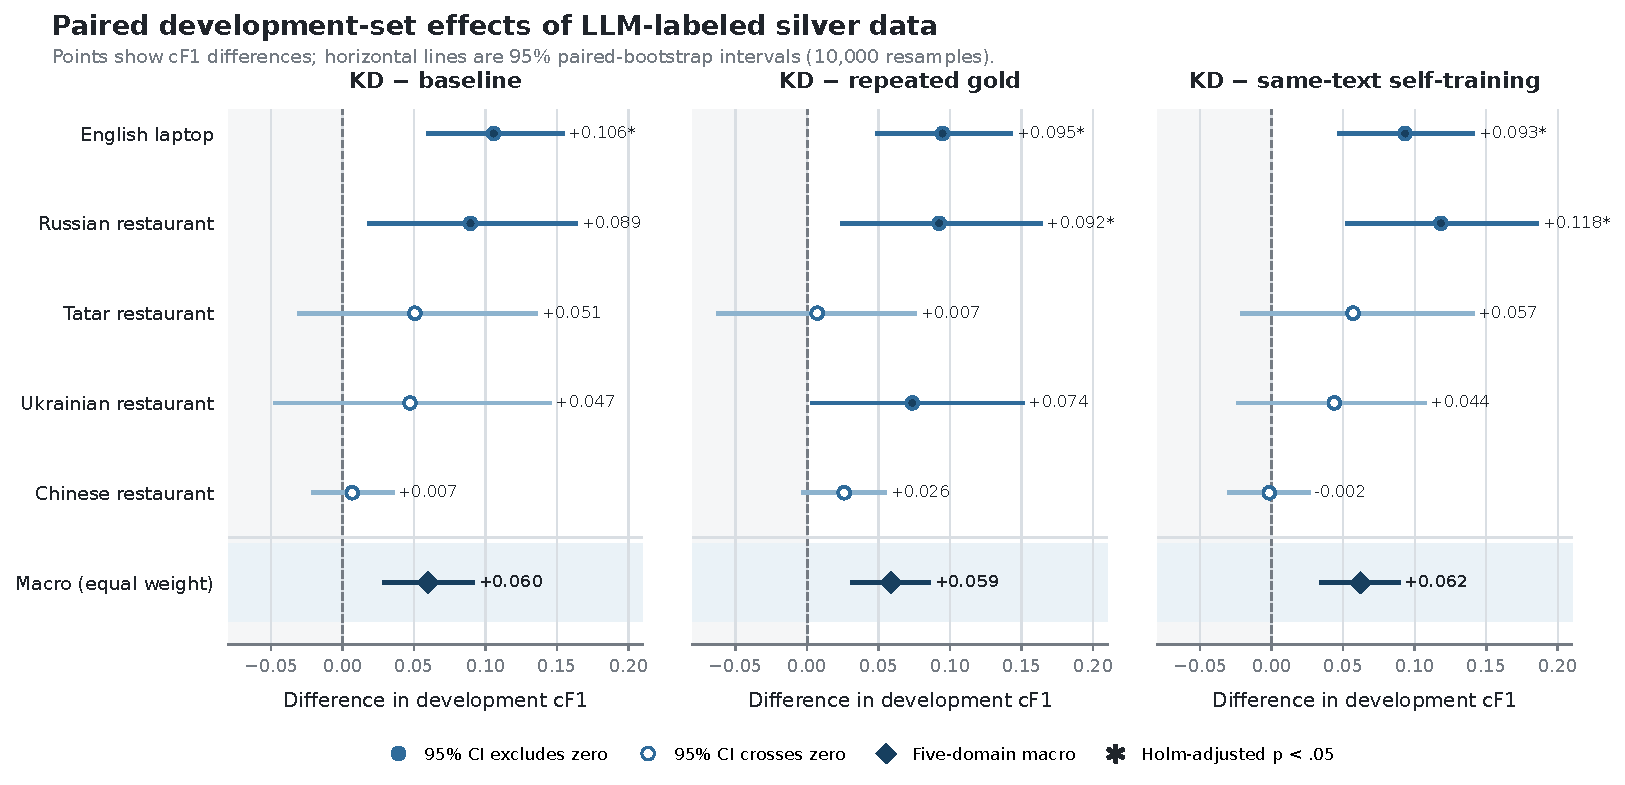
\includegraphics[width=\linewidth]{tallip_kd_effect_forest.pdf}
\caption{Development-set cF1 differences with 95\% paired-bootstrap intervals. Each panel uses the same five adopted datasets. The diamond is the equal-dataset-weight macro estimate; filled circles indicate an unadjusted interval that excludes zero, open circles are inconclusive, and a star marks a dataset comparison that remains significant after Holm correction within its five-comparison family.}
\Description{A three-panel forest plot compares knowledge distillation against the frozen baseline, repeated-gold exposure, and same-text self-training on five datasets. Diamonds show positive macro effects in all three panels. English laptop and Russian restaurant have the clearest positive dataset-level intervals; other intervals mostly cross zero.}
\label{fig:kd-effects}
\end{figure}

Table 5 summarizes the aggregate estimates and the number of
dataset-level comparisons supported before and after multiplicity
correction. KD exceeds the exposure-matched repeated-gold control by
+0.0588 {[}+0.0318,+0.0853{]} on average and the same-text self-training
control by +0.0621 {[}+0.0351,+0.0888{]}. By contrast,
self-training−repeated-gold is −0.0033 {[}−0.0226,+0.0170{]}, so the two
non-LLM controls have no reliable macro ordering.

{\small
\begin{longtable}[]{@{}
  >{\raggedright\arraybackslash}p{(\linewidth - 8\tabcolsep) * \real{0.1765}}
  >{\raggedleft\arraybackslash}p{(\linewidth - 8\tabcolsep) * \real{0.2353}}
  >{\raggedleft\arraybackslash}p{(\linewidth - 8\tabcolsep) * \real{0.2353}}
  >{\raggedright\arraybackslash}p{(\linewidth - 8\tabcolsep) * \real{0.1765}}
  >{\raggedright\arraybackslash}p{(\linewidth - 8\tabcolsep) * \real{0.1765}}@{}}
\caption{Fixed-task macro effects and dataset-level multiplicity summary.}
\label{tab:macro-effects}\\
\toprule
Contrast & Macro ΔcF1 & 95\% CI & Raw supported domains &
Holm-supported domains \\
\midrule
\endfirsthead
\caption[]{Fixed-task macro effects and dataset-level multiplicity summary
(continued).}\\
\toprule
Contrast & Macro ΔcF1 & 95\% CI & Raw supported domains &
Holm-supported domains \\
\midrule
\endhead
\bottomrule
\endlastfoot
KD−baseline & +0.0600 & {[}+0.0291,+0.0911{]} & eng, rus & eng \\
KD−repeated gold & +0.0588 & {[}+0.0318,+0.0853{]} & eng, rus, ukr &
eng, rus \\
KD−same-text self-training & +0.0621 & {[}+0.0351,+0.0888{]} & eng, rus
& eng, rus \\
Self-training$-$repeat-gold & −0.0033 & {[}−0.0226,+0.0170{]} & zho &
zho \\
\end{longtable}
}

The domain-level controls narrow the mechanism claim. For English and
Russian, LLM KD reliably exceeds both repeated-gold exposure and student
labels on the same texts, and these differences survive Holm correction.
Ukrainian KD exceeds repeated gold in the unadjusted comparison (+0.0736
{[}+0.0036,+0.1507{]}) but not after family-wise correction, and its
advantage over same-text self-training is inconclusive. Neither Tatar
nor Chinese restaurant establishes a reliable LLM-label advantage.
Chinese self-training itself exceeds repeated gold by +0.0276
{[}+0.0079,+0.0463{]}, which shows why an exposure control alone is
insufficient for attributing a gain to an LLM teacher.

\subsection{Teacher, Pool, and Quantity Do Not Admit a Universal
Ranking}\label{teacher-pool-and-quantity-do-not-admit-a-universal-ranking}

Table 6 summarizes the most controlled ablations and the boundary of
each inference. The direct teacher matrix supports greater overall
consistency for DeepSeek, but the matched Tatar downstream arm does not
support a universal teacher ordering. The Russian pool experiment
provides a clear within-domain ordering under a common teacher and cap,
while the Chinese observation points in a different direction under a
weaker control. Together, these results reject a universal pool-source
ranking rather than establishing that either generated or real text is
generally superior.

{\small
\begin{longtable}[]{@{}
  >{\raggedright\arraybackslash}p{(\linewidth - 6\tabcolsep) * \real{0.2500}}
  >{\raggedright\arraybackslash}p{(\linewidth - 6\tabcolsep) * \real{0.2500}}
  >{\raggedright\arraybackslash}p{(\linewidth - 6\tabcolsep) * \real{0.2500}}
  >{\raggedright\arraybackslash}p{(\linewidth - 6\tabcolsep) * \real{0.2500}}@{}}
\caption{Controlled ablations and allowed interpretation.}
\label{tab:ablations}\\
\toprule
Axis & Controlled comparison & Result & Allowed interpretation \\
\midrule
\endfirsthead
\caption[]{Controlled ablations and allowed interpretation (continued).}\\
\toprule
Axis & Controlled comparison & Result & Allowed interpretation \\
\midrule
\endhead
\bottomrule
\endlastfoot
Teacher fidelity & 8 datasets × identical label-hidden dev inputs &
DeepSeek higher in 8/8; supported in 3/8 & DeepSeek is more consistent
overall; no universal pairwise dominance claim \\
Teacher downstream & Tatar, same gold and 3,915 silver texts, five seeds
& DeepSeek−Qwen +0.0038 {[}−0.0823,+0.0852{]} & no reliable downstream
ranking difference \\
Pool source & Russian, same DeepSeek teacher and cap=3,000 & generated
.6162 \textgreater{} translated .5761 \textgreater{} real .5586 & strong
within-Russian ordering only \\
Pool source & Chinese restaurant, real vs generated & real−generated
+0.023 cF1 & observational; other factors are not fully matched \\
Silver quantity & Russian, same gen8k pool, seeds 42/123 &
cap3000−full7988 = −0.0114 mean & lower quantity does not explain the
independent gen4k advantage \\
Translation/native & Ukrainian pools differ in construction and quantity
& mixed & descriptive evidence only \\
\end{longtable}
}

The Russian same-pool quantity result failed the preregistered +1.5
percentage point continuation gate. We therefore did not train the other
three seeds or a cap5000 arm. The independent gen4k batch can outperform
the gen8k batch, but its advantage is more consistent with batch
composition, coverage, or labeling quality than with a general
preference for fewer silver rows. The evidence does not identify a
dose--response curve or an optimal cap.

\subsection{Complementarity Measurements Are Informative but Not a
Causal
Moderator}\label{complementarity-measurements-are-informative-but-not-a-causal-moderator}

The direct measurements in Table 7 provide counterexamples to a
single-metric explanation. English laptop has the largest observed
span-coverage expansion and the largest development gain. Chinese
restaurant has the highest direct DeepSeek fidelity in Table 3, yet it
has the smallest development gain and loses aspect and opinion span
coverage relative to its base data. Russian and Tatar show positive
downstream point estimates without a consistent increase in both span
inventories.

{\small
\begin{longtable}[]{@{}
  >{\raggedright\arraybackslash}p{(\linewidth - 10\tabcolsep) * \real{0.1304}}
  >{\raggedleft\arraybackslash}p{(\linewidth - 10\tabcolsep) * \real{0.1739}}
  >{\raggedleft\arraybackslash}p{(\linewidth - 10\tabcolsep) * \real{0.1739}}
  >{\raggedleft\arraybackslash}p{(\linewidth - 10\tabcolsep) * \real{0.1739}}
  >{\raggedleft\arraybackslash}p{(\linewidth - 10\tabcolsep) * \real{0.1739}}
  >{\raggedleft\arraybackslash}p{(\linewidth - 10\tabcolsep) * \real{0.1739}}@{}}
\caption{Descriptive complementarity and row-level error transitions.}
\label{tab:complementarity}\\
\toprule
Dataset & Silver rows & Span coverage Δ (aspect/opinion) & Category JSD Δ &
Repaired vs. harmed & KD$-$base cF1 \\
\midrule
\endfirsthead
\caption[]{Descriptive complementarity and row-level error transitions
(continued).}\\
\toprule
Dataset & Silver rows & Span coverage Δ (aspect/opinion) & Category JSD Δ &
Repaired vs. harmed & KD$-$base cF1 \\
\midrule
\endhead
\bottomrule
\endlastfoot
eng\_\allowbreak laptop & 7,547 & +21/+38 & −0.0141 & 71/44 & +0.1058 \\
rus\_\allowbreak restaurant & 3,000 & −4/+0 & +0.0503 & 20/19 & +0.0895 \\
tat\_\allowbreak restaurant & 3,915 & −9/+4 & +0.0571 & 16/20 & +0.0506 \\
ukr\_\allowbreak restaurant & 5,534 & +4/+9 & +0.0241 & 22/18 & +0.0472 \\
zho\_\allowbreak restaurant & 3,882 & −30/−56 & −0.0009 & 130/112 & +0.0069 \\
\end{longtable}
}

Across only five domains, teacher fidelity versus KD gain has Spearman
\(\rho=-0.70\) with a bootstrap interval of {[}−1.00,+0.875{]},
span-coverage gain versus KD gain has \(\rho=+0.70\) {[}−0.875,+1.00{]},
and category-alignment gain has \(\rho=+0.10\) {[}−1.00,+1.00{]}. The
intervals are too wide to establish a moderator. Slices by sentence
length, single versus multiple quads, rare category, and implicit aspect
or opinion are also heterogeneous. These measurements support a
multi-factor interpretation involving validity, coverage, distribution,
and teacher--student fit; they do not prove ``information
complementarity'' as a universal causal law.

\subsection{Frozen Official-Test Evaluation Supports Conditional
Generalization}\label{frozen-official-test-evaluation-supports-conditional-generalization}

Table 8 reports the one-shot post-competition evaluation. Among the five
preregistered KD contrasts, English, Russian, Tatar, and Ukrainian have
raw paired intervals above zero. Chinese restaurant has a negative point
estimate and an interval crossing zero. After Holm correction within
this five-contrast family, English, Tatar, and Ukrainian remain
significant; Russian does not.

{\small
\begin{longtable}[]{@{}
  >{\raggedright\arraybackslash}p{(\linewidth - 10\tabcolsep) * \real{0.1300}}
  >{\raggedright\arraybackslash}p{(\linewidth - 10\tabcolsep) * \real{0.2500}}
  >{\raggedleft\arraybackslash}p{(\linewidth - 10\tabcolsep) * \real{0.1200}}
  >{\raggedleft\arraybackslash}p{(\linewidth - 10\tabcolsep) * \real{0.1500}}
  >{\raggedleft\arraybackslash}p{(\linewidth - 10\tabcolsep) * \real{0.2200}}
  >{\raggedright\arraybackslash}p{(\linewidth - 10\tabcolsep) * \real{0.1300}}@{}}
\caption{Frozen main systems on official test and preregistered KD contrasts
(lap = laptop; rest = restaurant).}
\label{tab:official-test}\\
\toprule
Dataset & Frozen main system & Test cF1 & KD−baseline & 95\% CI &
Holm \textless{} .05 \\
\midrule
\endfirsthead
\caption[]{Frozen main systems on official test and preregistered KD contrasts
(continued; lap = laptop; rest = restaurant).}\\
\toprule
Dataset & Frozen main system & Test cF1 & KD−baseline & 95\% CI &
Holm \textless{} .05 \\
\midrule
\endhead
\bottomrule
\endlastfoot
eng-lap & clean DeepSeek KD & 0.3532 & +0.0822 &
{[}+0.0629,+0.1021{]} & yes \\
eng-rest & inherited V16 baseline & 0.5904 & --- & --- & --- \\
jpn-hotel & inherited V16 no-augmentation & 0.4217 & --- & --- & --- \\
rus-rest & DeepSeek gen4k KD & 0.5189 & +0.0211 &
{[}+0.0005,+0.0431{]} & no \\
tat-rest & Qwen KD & 0.4311 & +0.0274 & {[}+0.0071,+0.0482{]} &
yes \\
ukr-rest & clean DeepSeek KD & 0.4608 & +0.0393 &
{[}+0.0150,+0.0639{]} & yes \\
zho-lap & inherited V16 baseline & 0.4309 & --- & --- & --- \\
zho-rest & clean DeepSeek real-pool KD & 0.4660 & −0.0137 &
{[}−0.0289,+0.0014{]} & no \\
\end{longtable}
}

The test results strengthen the conclusion that KD can help under
selected domain conditions, but they do not support a five-domain
success claim. They also do not constitute a test-set model-selection
loop: all choices and prediction hashes were frozen before the labels
were retrieved, and no post-lock control was evaluated on official test.
None of the eight main systems exceeds the corresponding official
leaderboard best, so we make no test SOTA claim.

\section{Discussion}\label{discussion}

\subsection{Reliable Average Benefits Can Coexist with Domain-Level
Uncertainty}\label{reliable-average-benefits-can-coexist-with-domain-level-uncertainty}

The central empirical pattern is not that KD either works or fails
everywhere. Across the fixed five-domain set, KD has a positive macro
effect relative to the matched baseline, repeated-gold exposure, and
same-text student self-training. At the same time, the dataset-level
intervals differ markedly. English and Russian provide the strongest
development evidence that the LLM labels add information beyond both
non-LLM controls. Ukrainian provides weaker evidence: its
exposure-adjusted comparison is positive before, but not after,
family-wise correction, and its same-text teacher-source comparison
remains inconclusive. Tatar and Chinese restaurant do not establish a
reliable LLM-label advantage on development data.

These statements answer different questions. The macro bootstrap asks
whether the mean paired effect over the prespecified adopted-domain set
is positive when each dataset receives equal weight. A dataset-level
interval asks whether one domain independently supports the contrast. A
supported macro effect therefore does not imply five supported domain
effects, just as an inconclusive small-domain interval does not prove
that its true effect is zero. This distinction is especially important
for Russian, Tatar, and Ukrainian, whose development sets contain only
48 examples and consequently yield wide intervals.

The one-shot official-test results are consistent with conditional
rather than universal generalization. Four of five raw KD contrasts are
positive with intervals above zero, while three remain significant after
Holm correction. Chinese restaurant is an important counterexample: its
development ensemble has a small positive contrast, whereas its test
contrast is slightly negative and inconclusive. We therefore interpret
the aggregate result as evidence that offline LLM supervision can be
useful over the studied set, not as a guarantee for every language,
domain, or split.

Nor does the pattern support a simple low-resource rule. English laptop
has the largest development gain despite having more raw gold training
examples than the three 1,240-row Slavic/Turkic restaurant sets, while
the larger Chinese restaurant set shows the weakest adopted-KD contrast.
Gold size alone is not a sufficient predictor of benefit.

\subsection{Direct Fidelity Is a Screening Signal, Not a Sufficient
Selection
Rule}\label{direct-fidelity-is-a-screening-signal-not-a-sufficient-selection-rule}

Directly evaluating a teacher on label-hidden gold data removes a major
ambiguity in downstream-only studies. It reveals whether the teacher can
produce valid task structures and provides paired teacher comparisons
before student optimization is considered. The 8-by-2 experiment
indicates that DeepSeek is more consistent overall, but five of the
eight pairwise differences remain uncertain. The matched Tatar
experiment further shows that small downstream fluctuations cannot be
used to infer a reliable reversal in teacher quality.

Fidelity alone is nevertheless insufficient for selecting a complete KD
pipeline. Chinese restaurant illustrates the limitation most clearly: it
has the highest direct DeepSeek fidelity among the adopted domains, but
the smallest development gain and no supported official-test benefit.
Direct fidelity is measured on the gold development distribution,
whereas downstream training also depends on which texts enter the silver
pool, which categories and spans they cover, how their label
distribution interacts with the base data, and how the student responds
to the resulting mixture. A teacher can therefore label gold-like
examples accurately without supplying useful new supervision, or it can
add useful coverage even when its aggregate fidelity is not the highest.

The pool and quantity experiments reinforce this view. Under a common
Russian teacher and cap, generated, translated, and real pools have a
clear domain-local ordering. The observational Chinese comparison points
in the opposite direction, and the Russian same-pool cap intervention
shows that reducing the gen8k batch does not recover the separate gen4k
result. These findings favor a multi-factor account involving label
validity, pool composition, coverage, and teacher--student fit.
``Information complementarity'' is a useful description of that account,
but our measured proxies are not monotonic and were not independently
manipulated. It should not be treated as a proven universal moderator.

\subsection{An Audit-First Workflow Is More Defensible Than a Larger KD
Grid}\label{an-audit-first-workflow-is-more-defensible-than-a-larger-kd-grid}

The experiments suggest a practical workflow for multilingual and
low-resource structured prediction. First, a small label-hidden gold
probe should be used to measure candidate teachers directly, including
invalid, empty, \texttt{NULL}, rare category, span, and continuous-label
behavior. Second, every gold, augmented, pool, silver, and combined
training file should be audited against development and test using a
documented normalization key. Cleaning should be decided by the
inductive protocol, not by whether deletion improves the score.

Third, teacher, pool, and quantity decisions should be made within the
target domain under frozen development rules. A ranking learned on
Russian restaurant data should not be transferred to Chinese restaurant
without a matched test. Fourth, multiple training seeds and paired
example-level inference should be reported because seed variation and
evaluation-example variation answer different uncertainty questions.
Fifth, an exposure-matched control should be the minimum comparison when
silver data increases the number of training rows. Where feasible, the
stronger comparison is same-text self-training, which holds the
unlabeled text fixed and changes the supervision source. Finally, test
data should be used once, after checkpoint, threshold, and prediction
hashes are locked.

This workflow also provides a principled stopping rule. Once direct
fidelity, clean-inductive reruns, matched non-LLM controls, and frozen
evaluation agree on the boundary of the claim, adding more teacher,
pool, augmentation, or cap arms can increase multiplicity without
resolving the main uncertainty. The failed Russian quantity gate is an
example: stopping after the preregistered criterion failed is more
informative than completing a post-hoc curve and selecting its best
point.

\subsection{Offline Distillation Moves LLM Cost Out of Deployment but
Does Not Make Training
Free}\label{offline-distillation-moves-llm-cost-out-of-deployment-but-does-not-make-training-free}

The deployed system contains five student checkpoints and makes no LLM
calls. This separates annotation-time access to a large teacher from
inference-time operation and can be attractive when an API-based or
35B-parameter teacher is too costly or unavailable in production. In
retained development logs for the gold-repeat controls using the same
student configurations, the five-model ensembles process between 10.77
and 26.46 output rows per second in the CUDA model-forward loop,
depending on the dataset and inherited encoder. These rates exclude
checkpoint loading, tokenization setup, voting, and output serialization
and should not be interpreted as end-to-end KD latency benchmarks.

The evidence closure itself is computationally substantial. The 50
retained best checkpoints from the repeated-gold and self-training
controls occupy 301.54 GiB, and their recorded training logs sum to
134.98 run-wall hours on one RTX 4090, including checkpoint I/O. These
measurements document the cost of the study rather than a controlled
comparison between encoders, configurations, or storage devices.
Historical token-usage and provider-billing fields were not retained, so
we cannot reconstruct a defensible monetary cost for all silver
generation. Future experiments should store tokens, wall time, retries,
model revision, and billing metadata at collection time.

\subsection{Relation to the Prior ICONIP
Study}\label{relation-to-our-prior-iconip-study}

The ICONIP V20 work introduced the LEADER-DimASQP student. It also selected
encoder and training recipes by language and dataset and used five-seed
inference \citep{qin2026leader}. The present study reuses those components to hold
student capacity and decoding policy as stable as possible. It does not
claim Rethink, Hungarian matching, language-specific encoders, or
ensembling as new contributions.

The new research question is when LLM-labeled silver data improves that
fixed student and how such a claim can be audited. The evidence added
here---direct two-teacher fidelity across eight datasets, matched
teacher/pool/quantity comparisons, clean-inductive reruns, exposure and
same-text controls, multiplicity-aware paired inference, and a
dev-locked official-test evaluation---was not part of V20. This
distinction is methodological as well as editorial: architecture
improvements and silver-supervision effects are not pooled into one
attribution claim.

\section{Limitations and Ethical
Considerations}\label{limitations-and-ethical-considerations}

\subsection{Scope and Statistical
Power}\label{scope-and-statistical-power}

The study covers one structured sentiment task, six languages, eight
datasets, and three review domains. Direct fidelity uses all eight
datasets, but the downstream macro and control analyses are restricted
to five previously adopted KD systems. Those systems were selected
through earlier development work, so the macro estimand describes this
fixed adopted set rather than a random sample of languages or all eight
task datasets. In particular, the three non-adopted datasets do not have
comparable downstream KD controls and cannot be counted as negative or
positive KD evidence.

Several low-resource development sets contain only 48 examples. Paired
resampling preserves the available example-level uncertainty but cannot
create information that is absent from a small evaluation set. The
exploratory moderator analysis has only five domain-level observations;
its wide intervals preclude a reliable correlation claim. Larger
multilingual benchmarks and prospectively selected domains are needed to
test whether the present macro effect generalizes.

The official-test analysis is intentionally one-shot. Its family-wise
correction is a post-hoc robustness check, not a new selection
criterion, and the test results were not replicated across alternative
task collections. Although the lock prevents test-guided model selection
in this study, a future paper that chooses hypotheses based on these
released labels would require a new held-out evaluation source.

\subsection{Limits of Causal
Attribution}\label{limits-of-causal-attribution}

The repeated-gold control matches total row exposure, and the
self-training control additionally matches silver text and row count.
These comparisons remove important alternative explanations, but they do
not randomize every property of the training process. Student
pseudo-labels are produced by the repeated-gold ensemble, and
differences in label density, empty predictions, confidence, and error
structure remain part of the teacher-source treatment. The controls
therefore support statements about the complete supervision source, not
a claim that one isolated linguistic feature causes the gain.

Only the Russian pool comparison and Tatar teacher comparison closely
match the principal observable factors. The Chinese pool result and
Ukrainian translation/native result retain construction or quantity
differences and are descriptive. The Russian same-pool quantity
intervention uses two seeds because the preregistered continuation gate
failed; it rejects the proposed ``fewer is better'' explanation for that
pool but does not estimate a full dose--response. We also lack a
separate two-annotator human audit of newly generated Russian silver.
Direct fidelity against the official gold development labels remains the
main teacher-quality check.

\subsection{Model and Cost
Reproducibility}\label{model-and-cost-reproducibility}

We preserve prompts, raw responses, parsed outputs, requested and
returned model identities, timestamps, and hashes. Even so, an API model
name may refer to a service that changes after collection, and a local
quantized checkpoint may not behave identically under another runtime or
hardware stack. The teacher results should therefore be read as
evaluations of the recorded model endpoints and settings, not immutable
properties of the model families.

The resource audit is incomplete because historical token and monetary
billing were not stored. Logged wall time includes I/O and varies with
encoder, sequence composition, and checkpoint location. The reported
throughput covers only the model-forward loop. We consequently avoid
monetary, energy, and end-to-end latency comparisons that the retained
evidence cannot support.

\subsection{Bias, Data Governance, and Human
Oversight}\label{bias-data-governance-and-human-oversight}

LLM-generated labels can reproduce language, regional, cultural, and
domain biases from the teacher
\citep{cui2025bias,jadhav2025limitations}. This concern is particularly
important for Tatar and Ukrainian, where both teacher competence and
evaluation sample size are less certain than aggregate cF1 may suggest.
Automatic schema validation catches malformed spans and categories but
cannot guarantee that implicit opinions, intensity, or culturally
specific expressions are interpreted appropriately. Silver labels should
therefore augment, not silently replace, expert or native speaker review
in consequential applications.

Review text can also contain personal or sensitive content even when it
comes from a public corpus. Practitioners should verify dataset
licenses, provider terms, retention policies, and whether external API
processing is appropriate for their data. Private reviews should not be
sent to a third-party teacher without a suitable legal and governance
basis.

Finally, five-seed training and inference increase energy, storage, and
maintenance costs relative to a single student. Publishing stopped and
negative experiments reduces incentives to repeat uninformative sweeps,
while offline distillation eliminates teacher calls during deployment.
These benefits do not remove the need to evaluate whether the ensemble's
incremental accuracy justifies its operational footprint in a particular
application.

\section{Conclusion}\label{conclusion}

We studied offline structured LLM-to-student distillation for
multilingual DimASQP while fixing the inherited student architecture and
inference recipes. Across five adopted domains, KD has a reliable
positive macro effect relative to the matched baseline, exposure-matched
repeated gold, and labels produced by a student on the same silver
texts. Clean-inductive retraining, paired bootstrap inference, and a
frozen official-test evaluation show that this average benefit is not
solely an artifact of duplicated training exposure or known text
overlap.

The benefit is nevertheless domain-dependent. English and Russian
provide the clearest development evidence that LLM labels add value
beyond both non-LLM controls. Other domains remain uncertain under
matched comparisons, and Chinese restaurant does not show a supported
official-test gain. DeepSeek is more consistent in direct fidelity, but
the data do not establish a universal teacher ranking. Pool-source
results reverse across settings, and a same-pool Russian intervention
provides no support for a universal silver-size optimum.

The resulting lesson is methodological: silver supervision should be
selected and audited within domain. Direct teacher evaluation,
split-contamination checks, multiple seeds, matched exposure and
self-training controls, multiplicity-aware uncertainty, and a one-shot
test lock together provide a more credible basis for deciding when LLM
labels help. Future work should improve prospective measures of
supervision complementarity and evaluate them on new tasks and held-out
domains rather than extending post-hoc teacher or quantity grids.


\bibliographystyle{ACM-Reference-Format}
\bibliography{tallip_refs}

\end{document}
